\chapter{Metodología}
	
\tb{En los capítulos anteriores se ha presentado los distintos algoritmos de control y generación de trayectorias que se emplearñan para conseguir recorrer un circuito con un \tb{dron} de carreras autónomo }. En este apartado se presenta la metodología empleada para superar las pruebas clasificatorias del Alphapilot 2019 

\section{Sistemas de referencia}


\section{Generación de \textit{waypoints}}
Para recorrer el circuito de forma satisfactoria es necesario que la aeronave atraviese las distintas puertas o \textit{gates} que componen el circuito en un orden concreto. Para conseguir esto es necesario conocer las posiciones de las puertas en el mundo y generar los puntos de paso necesarios para que la aeronave pase a través de ellas sin colisionar.

En la competición se proporciona el orden en el que se deben atravesar las puertas y una posición aproximada de las posiciones de cada una de ellas en el mundo. 

\begin{figure}[htb!]
	\centering
	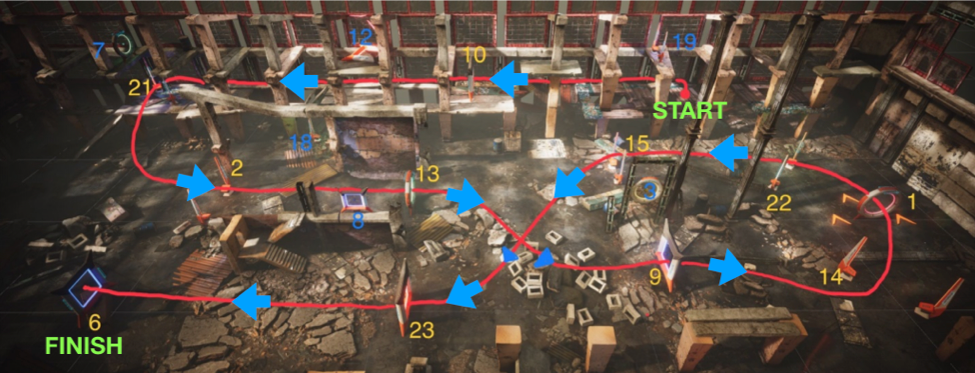
\includegraphics[width=\textwidth]{imagenes/diagramacircuito}
	\caption{Vista aérea del circuito en el simulador FightGoggles, las puertas que se deben traspasar se simbolizan con su número en color amarillo.}
	\label{waypoints:circuito}
\end{figure}

Como se puede observar en la figura \ref{waypoints:circuito} la aeronave debe recorrer 11 puertas, cada una con un número de identificación, en el orden indicado. 








\section{Trayectorias a largo y corto plazo}

